\documentclass[12pt]{article}
\usepackage{enumitem}
\usepackage{outlines}
\usepackage{amsfonts}
\usepackage{amssymb}
\usepackage{amsthm}
\usepackage{amsmath}
\usepackage{wrapfig}
\usepackage{float}
\usepackage{xcolor}
\usepackage{titlesec}
\usepackage{lipsum}
\usepackage{fancyhdr}
\pagestyle{fancy}
\usepackage{graphicx}
\usepackage{caption}
\usepackage{subcaption}

\newcommand{\tri}[2] {#1^{\Delta #2}}

\usepackage{tikz,tikz-3dplot}
\usetikzlibrary{scopes}
\usepackage{verbatim}

\tdplotsetmaincoords{70}{40}
 
 \renewcommand\refname{Bibliography}
 
\setcounter{secnumdepth}{4}
\titleformat{\paragraph}
{\normalfont\normalsize\bfseries}{\theparagraph}{1em}{}
\titlespacing*{\paragraph}
{0pt}{3.25ex plus 1ex minus .2ex}{1.5ex plus .2ex}


%\title{Some title containing the words ``triangular'', ``simplicial'', and
%``numbers'', e.g. this one}
%\date{\today}
%\author{Andrew Gleeson}
\begin{document}
\pagestyle{empty}
\begin{titlepage}
\begin{center}


\vspace*{3cm}

% Title

{ \huge \bfseries Triangular and Simplex Numbers \\[1cm] }

{ \large \bfseries An Introduction to Mathematical Thinking \\[3cm] }

{ \large Andrew Gleeson \\[3cm] }

% Author and supervisor
\begin{minipage}{0.4\textwidth}
\begin{flushleft} \large
\emph{Foundation:}\\[0.5cm]
Harutiun Nishanian\\[0.5cm]
Math 252
\end{flushleft}
\end{minipage}
\begin{minipage}{0.4\textwidth}
\begin{flushright} \large
\emph{Seminar:} \\[0.5cm]
Rob Komas\\[0.5cm]
Math 329
\end{flushright}
\end{minipage}

\vfill

% Bottom of the page
{\large \today}

\end{center}
\end{titlepage}

\vspace*{5cm}
\begin{abstract}

Triangular numbers are positive integers with properties related to
triangles.
Graphically, they can be represented as the number of points in $\mathbb{Z}^{2}$ bounded by a right isoceles triangle.  
They can also be viewed as $\sum_{i=1}^n i$, which is known to be  $\frac{n(n+1)}{2}$.
 Triangular numbers can be generalized to simplex numbers, which are analogous to triangular numbers in any dimension. 
 Triangular numbers show up often across various areas of mathematics, mostly in combinatorics. 
 Although some of the included results have been known for centuries, I
 independently arrived at many of the results. This paper describes the results,
 many of which can be shown though very elegant proofs, and my journey to them.
 Because triangular numbers are a relatively unknown but not overly complicated
 area of mathematics, they present an ideal opportunity to start real
 mathematical thinking.

\end{abstract}
\pagebreak
\pagestyle{plain}
\setcounter{page}{1}
\section{Introduction}

The concept of triangular numbers is fundamentally. Most people are very
familiar with square numbers ($n^2$), but we don't put much thought
into why a square is chosen as the shape (Figure ~\ref{square}). Geometrically, there are
other very interesting shapes. Two shapes that stand out are the
triangle, which has the least number of verticies required to bound an area in two-dimensional space, and the circle, which has an infinite
number of vertices. All other polygons are somewhere between the
two. So, it would seem that triangles, like squares, should be similarly important.
A square number can be thought of as the number of points is $\mathbb{Z}^2$ bounded by a square. They can also be viewed as $\sum_{i=1}^{n}n$ and $n^2$.



\begin{figure}[h]
\centering

\begin{subfigure}{0.4\textwidth}
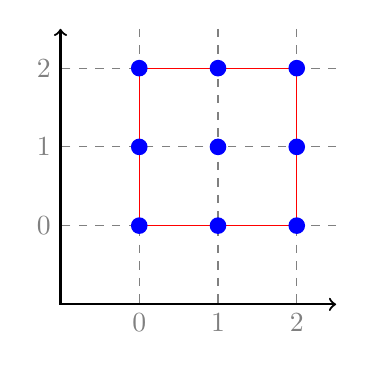
\begin{tikzpicture}
\foreach \x in {1,...,3}
     		\draw[dashed, gray] (\x,3.5) -- (\x,0)
			node[anchor=north] {\pgfmathparse{\x-1}\pgfmathprintnumber{\pgfmathresult}};		
\foreach \y in {1,...,3}
     		\draw[dashed, gray] (3.5,\y) -- (0,\y)
			node[anchor=east] {\pgfmathparse{\y-1}\pgfmathprintnumber{\pgfmathresult}};
\draw [<->, black, thick] (0,3.5) -- (0,0) -- (3.5,0);
\draw[red] (3,1) -- (3,3) -- (1,3) -- (1,1) -- cycle ;
\foreach \x in {1,...,3}
	\foreach \y in {1,...,3}
		\fill [blue] (\x, \y) circle [radius=3pt];
\end{tikzpicture}
\caption{$3^2 = 9$\label{square}}

\end{subfigure}
\begin{subfigure}{0.4\textwidth}
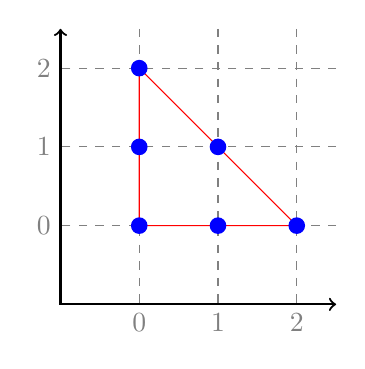
\begin{tikzpicture}
\foreach \x in {1,...,3}
     		\draw[dashed, gray] (\x,3.5) -- (\x,0)
			node[anchor=north] {\pgfmathparse{\x-1}\pgfmathprintnumber{\pgfmathresult}};			
\foreach \y in {1,...,3}
     		\draw[dashed, gray] (3.5,\y) -- (0,\y)
			node[anchor=east] {\pgfmathparse{\y-1}\pgfmathprintnumber{\pgfmathresult}};
\draw [<->, black, thick] (0,3.5) -- (0,0) -- (3.5,0);
\draw[red] (3,1) -- (1,3) -- (1,1) -- cycle ;
\fill [blue] (3, 1) circle [radius=3pt];
\fill [blue] (2, 1) circle [radius=3pt];
\fill [blue] (1, 1) circle [radius=3pt];
\fill [blue] (1, 2) circle [radius=3pt];
\fill [blue] (1, 3) circle [radius=3pt];
\fill [blue] (2, 2) circle [radius=3pt];
\end{tikzpicture}
\caption{$T_3 = 6$\label{triangular}}
%\vspace{-10pt}
\end{subfigure}
\caption{Graphic Representations}
\end{figure}

\section{Triangular Numbers}
To form a triangular number, we can instead bound the points with a right
isoceles triangle. (Figure ~\ref{triangular}) What would a triangular number be?
If we examine the triangular numbers, we can see that in each successive row, the number of dots increments by one. So, we can express the $n$th triangular number $T_n$ as the sum of the numbers 1 to $n$.\\
\\
$T_n = 1+2+...+n = \sum_{i = 1}^n i = \frac{n(n+1)}{2}$\\

With some simple steps, we can transform triangular numbers into something much more well known.

\begin{align*}
T_n &= \frac{n(n+1)}{2} \\
&= \frac{(n+1)!}{2! (n-1)!}\quad\text{(rewrite using factorials)}\\
&= \frac{k!}{2! (k-2)!} \quad\text{(let k = n+1)}\\
&= \binom{k}{2} \quad\text{(by the definition of a binomial coefficient)}\\
&= \binom{n+1}{2} \quad\text{(substitute)}
\end{align*}

In plain English, this means that the $n$th triangular number is the number of
combinations of 2 items from a set of n+1 items where order is unimportant and
repeats are culled. This countrasts to square numbers, where order
matters and repeats are allowed. This fact connects us to the world of
combinatorics.
However, I decided to not delve into combinatorics to find properties of triangular numbers. It is possible to manipulate already-known properties of binomial coefficients to say something about triangular numbers, but that would mean deviating from the beautiful geometry of triangular numbers. There exist many other properties of triangular numbers that have elegant geometric proofs, which was the path of interest to me.\\

For example, two important triangular identities are $T_n + T_{n-1} = n^2$ and
$T_n - T_{n-1} = n$. These identities are essential to the relationship between
triangular numbers and quadratic quantities. It means that any square number, or
any integer, can by represented as the sum or difference of two triangular numbers.

\begin{figure}[H]
\centering

\begin{centering}

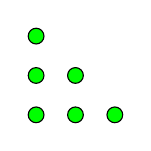
\begin{tikzpicture}[scale=0.5]
	\draw[fill=green] (0,0) circle [radius=0.2cm];
	\draw[fill=green] (0,1) circle [radius=0.2cm];
	\draw[fill=green] (0,2) circle [radius=0.2cm];
	\draw[fill=green] (1,0) circle [radius=0.2cm];
	\draw[fill=green] (1,1) circle [radius=0.2cm];
	\draw[fill=green] (2,0) circle [radius=0.2cm];
\end{tikzpicture}
\quad
\huge{+}
\quad
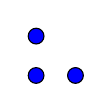
\begin{tikzpicture}[scale=0.5]
	\draw[fill=blue] (0,0) circle [radius=0.2cm];
	\draw[fill=blue] (1,0) circle [radius=0.2cm];
	\draw[fill=blue] (0,1) circle [radius=0.2cm];
\end{tikzpicture}
\quad
\huge{=}
\quad
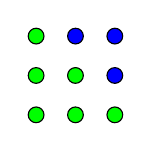
\begin{tikzpicture}[scale=0.5]
	\draw[fill=green] (0,0) circle [radius=0.2cm];
	\draw[fill=green] (0,1) circle [radius=0.2cm];
	\draw[fill=green] (0,2) circle [radius=0.2cm];
	\draw[fill=green] (1,0) circle [radius=0.2cm];
	\draw[fill=green] (1,1) circle [radius=0.2cm];
	\draw[fill=green] (2,0) circle [radius=0.2cm];
	
	\draw[fill=blue] (2,2) circle [radius=0.2cm];
	\draw[fill=blue] (2,1) circle [radius=0.2cm];
	\draw[fill=blue] (1,2) circle [radius=0.2cm];
\end{tikzpicture}
\end{centering}
\caption{$T_3 + T_2 = 3^2$\label{tnplustnminus1l}}
\end{figure}
\begin{figure}[H]
\centering

\begin{centering}

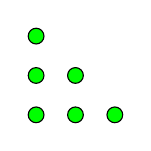
\begin{tikzpicture}[scale=0.5]
	\draw[fill=green] (0,0) circle [radius=0.2cm];
	\draw[fill=green] (0,1) circle [radius=0.2cm];
	\draw[fill=green] (0,2) circle [radius=0.2cm];
	\draw[fill=green] (1,0) circle [radius=0.2cm];
	\draw[fill=green] (1,1) circle [radius=0.2cm];
	\draw[fill=green] (2,0) circle [radius=0.2cm];
\end{tikzpicture}
\quad
\huge{-}
\quad
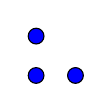
\begin{tikzpicture}[scale=0.5]
	\draw[fill=blue] (0,0) circle [radius=0.2cm];
	\draw[fill=blue] (1,0) circle [radius=0.2cm];
	\draw[fill=blue] (0,1) circle [radius=0.2cm];
\end{tikzpicture}
\quad
\huge{=}
\quad
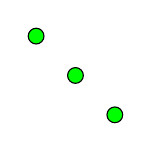
\begin{tikzpicture}[scale=0.5]
	%\draw[fill=green] (0,0) circle [radius=0.2cm];
	%\draw[fill=green] (0,1) circle [radius=0.2cm];
	\draw[fill=green] (0,2) circle [radius=0.2cm];
	%\draw[fill=green] (1,0) circle [radius=0.2cm];
	\draw[fill=green] (1,1) circle [radius=0.2cm];
	\draw[fill=green] (2,0) circle [radius=0.2cm];
	
	%\draw[fill=blue] (2,2) circle [radius=0.2cm];
	%\draw[fill=blue] (2,1) circle [radius=0.2cm];
	%\draw[fill=blue] (1,2) circle [radius=0.2cm];
\end{tikzpicture}
\end{centering}
\caption{$T_3 - T_2 = 3$\label{tnminustnminus1l}}
\end{figure}


\subsection{Properties}

Many properties of triangular numbers can be shown geometrically, while others are shown through the manipulation of equations.

For example, the identity $T_{2n} = 3\cdot T_n + T_{n-1}$ can be shown through a simple graphic.
\begin{figure}[H]
\centering

\begin{centering}

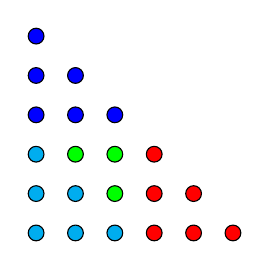
\begin{tikzpicture}
	\draw[fill=cyan] (0,0) circle [radius=0.1cm];
	\draw[fill=cyan] (0,0.5) circle [radius=0.1cm];
	\draw[fill=cyan] (0,1) circle [radius=0.1cm];
	\draw[fill=blue] (0,1.5) circle [radius=0.1cm];
	\draw[fill=blue] (0,2) circle [radius=0.1cm];
	\draw[fill=blue] (0,2.5) circle [radius=0.1cm];
	
	\draw[fill=cyan] (0.5,0) circle [radius=0.1cm];
	\draw[fill=cyan] (0.5,0.5) circle [radius=0.1cm];
	\draw[fill=green] (0.5,1) circle [radius=0.1cm];
	\draw[fill=blue] (0.5,1.5) circle [radius=0.1cm];
	\draw[fill=blue] (0.5,2) circle [radius=0.1cm];
	
	\draw[fill=cyan] (1,0) circle [radius=0.1cm];
	\draw[fill=green] (1,0.5) circle [radius=0.1cm];
	\draw[fill=green] (1,1) circle [radius=0.1cm];
	\draw[fill=blue] (1,1.5) circle [radius=0.1cm];
	
	\draw[fill=red] (1.5,0) circle [radius=0.1cm];
	\draw[fill=red] (1.5,0.5) circle [radius=0.1cm];
	\draw[fill=red] (1.5,1) circle [radius=0.1cm];
	
	\draw[fill=red] (2,0) circle [radius=0.1cm];
	\draw[fill=red] (2,0.5) circle [radius=0.1cm];
	
	\draw[fill=red] (2.5,0) circle [radius=0.1cm];
\end{tikzpicture}
\quad
\huge{$= 3\enspace\cdot$}
\enspace
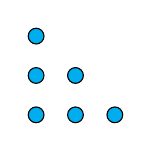
\begin{tikzpicture}
	\draw[fill=cyan] (0,0) circle [radius=0.1cm];
	\draw[fill=cyan] (0,0.5) circle [radius=0.1cm];
	\draw[fill=cyan] (0,1) circle [radius=0.1cm];
	
	\draw[fill=cyan] (0.5,0) circle [radius=0.1cm];
	\draw[fill=cyan] (0.5,0.5) circle [radius=0.1cm];
	
	\draw[fill=cyan] (1,0) circle [radius=0.1cm];
\end{tikzpicture}
\quad
\huge{+}
\quad
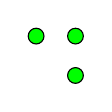
\begin{tikzpicture}

	\draw[fill=green] (0.5,1) circle [radius=0.1cm];
	
	\draw[fill=green] (1,0.5) circle [radius=0.1cm];
	\draw[fill=green] (1,1) circle [radius=0.1cm];
\end{tikzpicture}
\end{centering}
\caption{$T_{6} = 3 \cdot T_3 + T_2$ \cite{nelsen} \label{T2n}}
\end{figure}

These properties are integral to building the intuition and machinery
necessary to derive more complicated identities. Being able to visualize
triangular numbers leads one to make non-trivial connections that are
not apparent in the algebra. However, some identities do lend themselves to an
algebraic derivation.

\begin{enumerate}
  \item $(T_n)^2 = \sum_{i=1}^n i^3$
  \item $T_{a+b} = T_a + T_b + 2ab$
  \item $T_{ab} = T_a T_b + T_{a-1}T_{b-1}$
  \item $T_n - T_{n-k} = \frac{k}{2} (2n + 1 - k)$
  \item All even perfect numbers (a number which equals the sum of its proper
  divisors excluding itself) are triangular numbers. \cite{tanton}
\end{enumerate}

And , by using (4), it can be shown that the difference of two triangular numbers will never be a perfect square if $k$ is two or greater.\\

Some other identities are even more obscure. Gauss, with his Eureka Theorem,
showed that any integer is the sum of at most three triangular numbers. \cite{bell} There is
no known elementary proof of this, showing a connection to deeper mathematics.


\subsubsection{Reciprocal Infinite Series}

There is a nice cleanliness to the reciprocal sum of all triangular numbers. By a simple telescopic series, $\sum_{n=1}^{\infty} \frac{1}{T_n} = 2$.

Since $\frac{1}{T_n} = \frac{2}{n(n+1)}$ can be rewritten as
$\frac{2}{n}-\frac{2}{n+1}$ by partial fractions, it follows that

\begin{align*}
\sum_{n=1}^{\infty} \frac{1}{T_n} = \sum_{n=1}^{\infty} \frac{2}{n} -
\frac{2}{n+1}
\end{align*}

If we write out the first few term, we begin to see a pattern:

\begin{align*}
\sum_{n=1}^{\infty} \frac{1}{T_n} = 
\left[ \frac{2}{1} - \frac{2}{2} \right] +
\left[ \frac{2}{2} - \frac{2}{3} \right] +
\left[ \frac{2}{3} - \frac{2}{4} \right] +
\ldots
\end{align*}

It appears that the first part of each term cancels the second part of the
previous term. Because they cancel out in pairs, we are left with

\begin{align*}
\sum_{n=1}^{\infty} \frac{1}{T_n} = 2 - \lim_{n \to \infty} \frac{2}{n+1}
\end{align*}

Because the limit of $\frac{2}{n+1}$ as $n$ goes to infinity is zero, we are
left with the exceedingly simple 

\begin{align*}
\sum_{n=1}^{\infty} \frac{1}{T_n} = 2
\end{align*}

Some mathematicians looked at subseries of this, expanding it to the form $T_{mn+r}$ instead of just $T_n$.
\cite{bruckman} They found that
\begin{multline*}
		\sum_{n=0}^\infty \frac{1}{T_{mn+r}} = 
		\frac{2}{m} \sum\limits_{0<j<m/2} \left\{ 
		\left[
			\cos \left(\frac{2 \pi j (r+1)}{m} \right) - \cos \left( \frac{2 \pi j r}{m} \right)
		\right] \right. \\
		\left. \cdot \ln \left[ 
		2 - \cos \left( \frac{2 \pi j}{m} \right)
		\right]
		- \left[ \sin \left(\frac{2 \pi j (r+1)}{m} \right) - \sin \left( \frac{2 \pi j r}{m} \right) \right] \right. \\
		\left. \cdot \frac{\pi (m - 2j)}{m}
		\right\} + 2 \delta_{mr} + \varepsilon_m \cdot (-1)^{r+1} 2 \ln(2)
\end{multline*}

Note: $\delta_{mr}$ is the Kronecker delta function, which is 1 when $m=r$ and
0 otherwise. $\varepsilon_m$ returns 1 if $m$ is even, and 0 if $m$ is odd.\\

Plugging in specific $m$ and $r$:

\begin{itemize}
	\item $\sum_{n=0}^\infty \frac{1}{T_{2n+2}} = 2 - 2 \ln 2$
	\item $\sum_{n=0}^\infty \frac{1}{T_{3n+1}} = \frac{2 \pi \sqrt{3}}{9}$
	\item $\sum_{n=0}^\infty \frac{1}{T_{4n+1}} = \frac{\pi}{4} + \frac{3}{2}\ln 2$
	\item $\sum_{n=0}^\infty \frac{1}{T_{4n+2}} = \frac{\pi}{4} - \frac{3}{2}\ln 2$
	\item $\sum_{n=0}^\infty \frac{1}{T_{4n+3}} = - \frac{\pi}{4} + \frac{5}{2}\ln 2$
\end{itemize}

These results cannot be proven without complex analysis and other
specialized tools, revealing a deeper connection to higher mathematics that is
not intuitively obvious. See Appendix A for an explanation of how they follow
from the given formula. However, a brute-force numerical analysis I carried out
confirms them to my satisfaction.
\iffalse
\paragraph{Example  - $T_{2n+2}$}

\begin{align*}
\sum_{n=0}^\infty \frac{1}{T_{2n+2}} = 
		\frac{2}{2} \sum\limits_{0<j<2/2} \left\{ 
		\left[
			\cos \left(\frac{2 \pi j (2+1)}{2} \right) - \cos \left( \frac{2 \pi j (2)}{2} \right)
		\right] \right. \\
		\left. \cdot \ln \left[ 
		2 - \cos \left( \frac{2 \pi j}{2} \right)
		\right]
		- \left[ \sin \left(\frac{2 \pi j (2+1)}{2} \right) - \sin \left( \frac{2 \pi j (2)}{2} \right) \right] \right. \\
		\left. \cdot \frac{\pi (2 - 2j)}{2}
		\right\} + 2 \delta_{2,2} + \varepsilon_2 \cdot (-1)^{2+1} 2 \ln(2)\\
		\\
		= 2 \delta_{2,2}-\varepsilon_{2} \cdot 2 \ln 2\\
		= 2 \cdot 1 - 1\cdot 2 \ln 2\\
		= 2 - 2 \ln 2
\end{align*}
\fi
\paragraph{Example  - $T_{3n+1}$}

\begin{align*}
		\sum_{n=0}^\infty \frac{1}{T_{3n+1}} = 
		\frac{2}{3} \sum\limits_{0<j<3/2} \left\{ 
		\left[
			\cos \left(\frac{2 \pi j (1+1)}{3} \right) - \cos \left( \frac{2 \pi j (1)}{3} \right)
		\right] \right. \\
		\left. \cdot \ln \left[ 
		2 - \cos \left( \frac{2 \pi j}{3} \right)
		\right]
		- \left[ \sin \left(\frac{2 \pi j (1+1)}{3} \right) - \sin \left( \frac{2 \pi j (1)}{3} \right) \right] \right. \\
		\left. \cdot \frac{\pi (3 - 2j)}{3}
		\right\} + 2 \delta_{3,1} + \varepsilon_3 \cdot (-1)^{1+1} 2 \ln(2)\\
		\\
		= \frac{2}{3} \left\{ 0 - [-\sqrt{3}] \cdot \frac{\pi}{3} \right\} + 2 \cdot 0 + 0 \cdot 2 \ln 2\\
		= \frac{2 \pi \sqrt{3} }{9}
\end{align*}

At the very least, it is remarkable that there are several similar terms in the results.

\section{Simplex Numbers}
\begin{figure}[H]
\centering

\begin{centering}
\def\s{2} % F_g

\begin{tikzpicture}[>=stealth,tdplot_main_coords]
    	\coordinate (O) at (0,0,0);
   	\coordinate (A) at (0,\s,0);
   	\coordinate (B) at ({sqrt(3)/2*\s},{\s/2},0);
	\coordinate (C) at ({sqrt(3)/6*\s},{\s/2},{sqrt(6)/3*\s});
    
    	%\draw[->] (O) -- (6,0,0);
    	%\draw[->] (O) -- (0,6,0);
    	%\draw[->] (O) -- (0,0,6);
    
    	
    	\draw[blue,fill=yellow!50] (O) -- (A) -- (B) -- cycle;
    	\draw[blue,fill=red!20] (O) -- (A) -- (C) -- cycle;
    	
    	\draw[blue,fill=green!10] (A) -- (B) -- (C) -- cycle;
    	
    	\draw[fill=red]  ($(A)!0.5!(B) $)  circle [radius=0.075cm];
    	\draw[fill=blue]  ($(A)!0.5!(C) $)  circle [radius=0.075cm];
    	\draw[fill=red]  ($(O)!0.5!(A) $)  circle [radius=0.075cm];
    	
    	\draw[fill=red] (A) circle [radius=0.1cm];
    	\draw[blue,fill=blue!10,opacity=0.6] (O) -- (B) -- (C) -- cycle;

	\draw[fill=red] (O) circle [radius=0.1cm];
    	
    	\draw[fill=red] (B) circle [radius=0.1cm];
    	\draw[fill=green] (C) circle [radius=0.1cm];
    	
    	
    	\draw[fill=red]  ($(O)!0.5!(B) $)  circle [radius=0.075cm];
    	\draw[fill=blue]  ($(O)!0.5!(C) $)  circle [radius=0.075cm];
    	
    	\draw[red, thick] (O) -- (B) -- (A) -- cycle;
    	\draw[blue, thick] ($(A)!0.5!(C) $) -- ($(C)!0.5!(B) $) --($(C)!0.5!(O) $) -- cycle;
    	
    	
    	
    	\draw[fill=blue]  ($(C)!0.5!(B) $)  circle [radius=0.075cm];
    	
\end{tikzpicture}


\huge{$\Downarrow$}\\

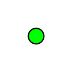
\begin{tikzpicture}
	\draw[fill=green] (0,0) circle [radius=0.1cm];
\end{tikzpicture}\\
\huge{+}\\
\vspace{0.3cm}
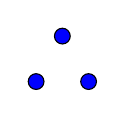
\begin{tikzpicture}
	\draw[fill=blue] (0,0) circle [radius=0.1cm];
	\draw[fill=blue] ({1*2/3},0) circle [radius=0.1cm];
	\draw[fill=blue] ({1/2*2/3},{sqrt(3)/2*2/3}) circle [radius=0.1cm];
\end{tikzpicture}\\
\huge{+}\\
\vspace{0.3cm}
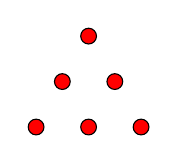
\begin{tikzpicture}
	\draw[fill=red] (0,0) circle [radius=0.1cm];
	\draw[fill=red] (2/3,0) circle [radius=0.1cm];
	\draw[fill=red] ({1/2*2/3},{sqrt(3)/2*2/3}) circle [radius=0.1cm];
	\draw[fill=red] ({-1/2*2/3},{-sqrt(3)/2*2/3}) circle [radius=0.1cm];
	\draw[fill=red] ({1/3},{-sqrt(3)/3}) circle [radius=0.1cm];
	\draw[fill=red] ({3/3},{-sqrt(3)/3}) circle [radius=0.1cm];
\end{tikzpicture}
\end{centering}
\caption{$\tri{3}{3}= 10$\label{tetrahedral}}
\end{figure}

Triangular numbers can be generalized to any dimension by turning them into simplexes. A simplex is a generalization of the idea of a triangle or tetrahedron to any dimension. For example, a triangle is a 2-simplex, meaning a simplex in two dimensions. A tetrahedron is a 3-simplex - and the list goes on. I will use the notation $\tri{n}{d}$ to signify the $n$th $d$-simplex number.

\subsection{Tetrahedral Numbers}
We have cube numbers, ($n^3$ or $\sum_{i=1}^{n}n^2$) --- what would tetrahedral numbers be? (Figure ~\ref{tetrahedral}) In the same way that a cube is made up of squares, a tetrahedral number is the sum of triangular numbers.

$\tri{n}{3} = \tri{1}{2}+\tri{2}{2}+...+\tri{n}{2} = \sum_{i=1}^n \tri{i}{2} = \frac{n(n+1)(n+2)}{6}$

I spent a great amount of time working with tetrahedral numbers, because the
concreteness of the graphical interpretation was very helpful for me. However,
it does have its limits -- for example, I attempted to visualize the
multiplication of a triangular number and a scalar as a prism, which turned out
to be fruitless.

\subsection{Fourth dimension and beyond}
Many of the properties of triangular and tetrahedral numbers hold true for any
arbitrary dimension. It was natural for me to ask the same questions as I did
about triangular numbers. For example, there is a pattern that the simplex
number in each dimension is a sum of the smaller dimensions. Geometrically, a
triangle is made out of three lines. A tetrahedron is bounded by
four triangles.  It would make sense, then, that a 4-simplex would in some
sense be comprised of tetrahedra. Numerically, we saw that $\tri{n}{2}$ is the
sum from 1 to n, and that $\tri{n}{3}$ was the sum of the first $n$ triangular numbers. This carries over:
\begin{align*}
\tri{n}{d} &= \sum_{i=1}^n \tri{i}{d-1}
\end{align*}
The combinatoric identity also generalizes:
\begin{align*}
 \tri{n}{d} = \binom{n+d-1}{d}
 \end{align*}
 
 The reciprocal infinite sum generalizes wonderfully, giving us
 \begin{align*}
 \sum_{n=1}^{\infty} \frac{1}{\tri{n}{d}} = \frac{d}{d-1}
  \end{align*}
 However, some properties do not translate easily. The square identity, $n^2 =
 T_n + T_{n-1}$, is very simple. Unfortunately, one identity derived graphically
 is significantly more complex for cubes:
 
 \begin{align*}
 n^3 = \tri{n}{3} + \tri{(2n-2)}{3} - 3 \tri{(n-2)}{3}
 \end{align*}
 
 This can be shown by visualizing tetrahedral numbers as the sum of triangular
 numbers, and cubes as the sums of square numbers. Although the proof is
 relatively simple, find this property took a considerable amount of graphical
 intuition and induction. On the other hand, an algebraic combination of
\begin{align}
  T_n + T_{n-1} = n^2\\
  T_n - T_{n-1} = n
\end{align}
by multiplication gives us:
\begin{align*}
	(T_n)^2 - (T_{n-1})^2 = n^3
\end{align*}
 
 Unfortunately, multiplication of triangular number does not lend itself to
 a convenient graphical interpretation.
 
 \subsubsection*{Symbolic Proof}
 \begin{multline*}
 \tri{n}{3} + \tri{(2n-2)}{3} - 3 \tri{(n-2)}{3} =\\
= \frac{(n)(n+1)(n+2)}{6} + \frac{(2n-2)(2n-1)(2n)}{6} - \frac{3(n-2)(n-1)(n)}{6}\\
= \frac{n^3 + 3n^2 + 2n}{6} + \frac{ 8n^3 - 12n^2 + 4n}{6} - \frac{3n^3 - 9n^2 + 6n}{6}\\
= \frac{n^3 + 3n^2 + 2n + 8n^3 - 12n^2 + 4n - 3n^3 + 9n^2 - 6n}{6}\\
= \frac{6n^3}{6} = n^3
 \end{multline*}
 
 \section{Conclusion}

Hopefully, you agree that triangular and simplex numbers are interesting.
Although the concept of a triangular number is exceedingly simple, they have a
surprisingly broad scope and a powerful geometric appeal. Many of the results
have a certain symmetry that falls from the underlying simplicity of the
concept. Additionally, and more informally, following the triangular trail was a
great deal of fun. Because triangular and simplicial numbers are relatively
obscure, I was only able to find citations for many results after I knew exactly
what I was looking for -- that is, I independently derived them. This research
required me to do a great deal of mathematical thinking, which will not be found
in most math classes. The beauty of triangular numbers lies in the ease with
which they lend themselves to the independent derivation of properties. In much
of mathematics, you must spend years taking classes, building intuition and
machinery, before being able to discover results for yourself without knowing
the answer ahead of time, or even if an answer exists. The machinery of
triangular numbers is sticks and stones -- algebra is enough to
understand most of the properties. This allowed me to jump into the discovery
phase very quickly. In a sense, the obscurity of triangular numbers is a
boon. There are no books to read about triangular numbers -- you bring all your
tools to the table yourself. You need to wrangle results out yourself. Isn't
that what mathematical thinking is? The plug-and-chug method does no one any
favors -- a computer will always outperform a human in raw computation and rote
memorization. Mathematical advances are driven by imagination, and the
heuristic process. I think working with triangular and simplex numbers helps to
further this ablity.

\pagebreak
\appendix

\section{Proof of the Tetrahedral Number Formula}
\subsection*{Inductive proof of the tetrahedral number formula}

Let $F(n)$ be the $n$th tetrahedral number, and $g(n)$ be the $n$th trianhular
number. By definition, $F(n) = g(1)+g(2)+g(3)+\ldots+g(n)$

\subsubsection*{Claim}
\begin{align*}
F(n) = \frac{n(n+1)(n+2)}{6}
\end{align*}

\subsubsection*{Proof: Induction on $n$}
\quad\textbf{n=1}
\begin{align*}
F(1)=g(1)=1\\
F(1)=\frac{(1)(2)(3)}{6}=1
\end{align*}
\quad\textbf{Inductive Step}\\

Assume $F(k) = \frac{k(k+1)(k+2)}{6}$. We want to show that $F(k+1) =
\frac{(k+1)(k+2)(k+3)}{6}$
\begin{align*}
F(k + 1) =  g(1) + g(2) + g(3) + \cdots + g(k) + g(k+1)\\
	 F(k + 1) =  F(k) + g(k+1)\\
	 F(k + 1) =   \frac{k(k+1)(k+2)}{6} + \frac{(k+1)(k+2)}{2}\\
	 F(k + 1) =   \frac{k(k+1)(k+2)}{6} + \frac{3(k+1)(k+2)}{6}\\
	 F(k + 1) =   \frac{k(k+1)(k+2) + 3(k+1)(k+2)}{6}\\
	 F(k + 1) =   \frac{(k+1)(k+2) (k+3)}{6}
\end{align*}

\begin{center}$\therefore F(n) = \frac{n(n+1)(n+2)}{6}$ \end{center}
\subsection*{Deductive proof of the tetrahedral number formula}
\subsubsection*{Proof}

%\begin{proof}

%\end{proof}

\begin{enumerate}
	\item Let $g(n)$ be the $n$th triangular number.

		$g(n) = \frac{n(n+1)}{2}$
	\item Let $F(n)$ be the $n$th tetrahedral number.
	
		$F(n) = \sum\limits_{i=1}^n g(i)$
	\item Substitute:
		
		$F(n) = \sum\limits_{i=1}^n \frac{i(i+1)}{2}$
	\item Distribute:
	
		$F(n) = \sum\limits_{i=1}^n \frac{i^2}{2} + \frac{i}{2}$
	\item Split:
	
		$F(n) = \sum\limits_{i=1}^n \frac{i^2}{2} + \sum\limits_{i=1}^n \frac{i}{2}$
	\item Take out constants:
	
		$F(n) = \frac{1}{2} \sum\limits_{i=1}^n i^2 + \frac{1}{2} \sum\limits_{i=1}^n i$
	\item Substitute known formulas for sums:
	
		$F(n) = \frac{1}{2} \left( \frac{n(n+1)(2n+1)}{6} + \frac{n(n+1)}{2} \right) $
	\item Add:
	
		$F(n) = \frac{1}{2} \left( \frac{n(n+1)(2n+1) + 3n(n+1)}{6} \right) $
	\item Factor:
	
		$F(n) = \frac{1}{2} \left( \frac{n(n+1) ((2n+1) + 3))}{6} \right) $
	\item Simplify:
	
		$F(n) = \frac{1}{2} \left( \frac{n(n+1) (2n+4 )}{6} \right) $
	\item Simplify:
	
		$F(n) = \frac{1}{2} \left( \frac{2n(n+1) (n+2 )}{6} \right) $

\end{enumerate}

\begin{center}$\therefore F(n) = \frac{n(n+1)(n+2)}{6}$ \end{center}

\pagebreak
\begin{thebibliography}{8}
\bibitem{bell}
	Bell, Eric Temple.  ``Gauss, the Prince of Mathematicians''. In Newman, James R. The World of Mathematics I. Simon \& Schuster. (1956): 295�339. 


  
 \bibitem{bruckman}
 	Bruckman, Paul, Joseph B. Dence, Thomas P. Dence, and Justin Young. ``Series of Reciprocal Triangular Numbers.'' The College Mathematics Journal 44.3 (2013): 177-84.
 
 \bibitem{fang}
 	Fang, Jin-Hui. "Nonexistence of a Geometrical Progression That Contains Four Triangular Numbers." Electronic Journal of Combinatorial Number Theory 7 (2007).

 	
 \bibitem{nelsen}
 	 Nelsen, Roger B. Proofs without Words: Exercises in Visual Thinking. Washington, D.C.: Mathematical Association of America, 1993.
 	 
\bibitem{oeis1}
	OEIS Foundation Inc. (2011), The On-Line Encyclopedia of Integer Sequences, http://oeis.org/A000217.
	
\bibitem{oeis2}
	 OEIS Foundation Inc. (2011), The On-Line Encyclopedia of Integer Sequences, http://oeis.org/A000292.

\bibitem{tanton}
  Tanton, James. ``A Dozen Questions about Triangular Numbers.'' Math Horizons 13 (2005).

\bibitem{ulas}
 	Ulas, Maciej. "On Certain Diophantine Equations Related to Triangular and Tetrahedral Numbers." {\tt arXiv:0811.2477v1 [math.NT]}
\end{thebibliography}
\end{document}